% Created 2018-04-14 Sat 21:09
\documentclass[11pt]{article}
\usepackage[utf8]{inputenc}
\usepackage[T1]{fontenc}
\usepackage{fixltx2e}
\usepackage{graphicx}
\usepackage{longtable}
\usepackage{float}
\usepackage{wrapfig}
\usepackage{rotating}
\usepackage[normalem]{ulem}
\usepackage{amsmath}
\usepackage{textcomp}
\usepackage{marvosym}
\usepackage{wasysym}
\usepackage{amssymb}
\usepackage{hyperref}
\tolerance=1000
\usepackage{palatino}
\usepackage[top=1in, bottom=1.25in, left=1.25in, right=1.25in]{geometry}
\usepackage{setspace}
\setcounter{secnumdepth}{1}
\author{PRAVEEN KUMAR R}
\date{16-29 March 2018 (Mon-Thurs)}
\title{Exercise 9: Recursion}
\hypersetup{
  pdfkeywords={},
  pdfsubject={},
  pdfcreator={Emacs 24.5.1 (Org mode 8.2.10)}}
\begin{document}

\maketitle
\linespread{1.2}
\begin{center}
\begin{tabular}{lr}
Assignment & 9\\
Reg No & 312217104114\\
Name & PRAVEEN KUMAR R\\
Grade & \\
Date & 29-03-2018\\
\end{tabular}
\end{center}
\linespread{1.5}

\section{Text processing}
\label{sec-1}
Read a text from stdin. Define functions for doing each of
the following operations. Test the functions individually.
\begin{enumerate}
\item Store the lines in as an array of lines, each line a C-string.
\item Store each line as an array of words, each word a C-string.
\item Count the number of lines.
\item Count the number of words.
\item Define a function to ``search and replace'' a word by another word.
\item Capitalize the first letter of each line.
\end{enumerate}

\subsection*{algorithm development:}
\label{sec-1-1}
\begin{itemize}
\item \textbf{storing lines as array of lines}
since the delimiter for scanf is a white space lines cannot be
read from stdin by scanf. Therefore fgets is used read the input.
\item \textbf{Store each line as an array of words, each word a C-string}
Considering the fact that each words are separated by a white space
each line is analysed and broken down in to words
\item \textbf{Count the number of lines and Count the number of words.}
Since the lines and words are already separated and stored in an array 
the number of elements  in the array will be the number of lines and words
in given text.
\item \textbf{search and replace}
Each word in the text is compared with the word that is to be replaced and 
when the word to be replaced is found the word is replaced with new word.
\item \textbf{capitalise}
A loop is used to traverse through all elements in the array and
first character of each line is capitalised.
\end{itemize}
\subsection*{program design}
\label{sec-1-2}

\subsection*{program}
\label{sec-1-3}

\begin{verbatim}
#include<stdio.h>
#include<stdlib.h>
#include<string.h>

/* input: k: an array of character pointers whose last pointer is pointed to NULL
	  s: a c string which is to be searched
	  r: a c string which is to be replaced wih
   output
       modified array of pointers.
*/ 
int search(char* k[],char s[],char r[])
{
int i=0,j=0,p=0,h=0;
char l[300],word[20],newline[300];
strcpy(newline,"");
while(k[h]!=NULL)
  {
    i=0;
    strcpy(l,k[h]);
    while(i<strlen(l))
     {
	 while(l[i]!=' '&&l[i]!='\0')
	   {
		word[j++]=l[i++];
	   }
	 word[j]='\0';
	 if(strcmp(word,s)==0)
	   {
		strcpy(word,r);
	   }
	 strcat(word," ");
	 strcat(newline,word);
	 j=0;
	 i++;
     }
    printf("%s \n",newline);
    k[h]=(char*) malloc(sizeof(newline));
    strcpy(k[h],newline);
    strcpy(newline,"");
    h++;       
  }
return 0;
}
/* input: p: an array of character pointer whose last pointer is pointed to NULL
   output: capitalise the first letter of each line.
*/

void capitalise(char* p[])
{
  int i=0;
  while(p[i])
    {
      char k=p[i][0];
      p[i][0]=toupper(k);
      i++;
     }

}
/*
 input: k: an array of character pointers whose last pointer is pointed to NULL
 output: number of elements in k
*/ 
int count_lines(char* k[])
{
  int count=0;
  for(;k[count];count++);
  return count;
}
/*
 input: k: an array of character pointers whose last pointer is pointed to NULL
	c: an empty array of character pointers.
 output: 
	each word in k is a element in c (a c-string)
*/ 
void store_words(char* k[],char* c[])
{ 
int i=0,j=0,p=0,h=0;
char l[300],word[20];
while(k[h]!=NULL)
  { i=0;
    strcpy(l,k[h]);
    while(i<strlen(l))
     { while(l[i]!=' '&&l[i]!='\n'&&l[i]!='\0')
	 word[j++]=l[i++];
     word[j]='\0';
     c[p]=(char*) malloc(sizeof(word));
     strcpy(c[p],word);
     p++;
     j=0;
     i++;
    }  
    h++;       
  }
c[p]=NULL;

}
/* 
   input: c: an array of charater pointers hose last element is NULL
   output: number of words in c
*/
int count_words(char *c[])
 {
   char *k[200];
   store_words(c,k);
   return count_lines(k);
 }
void print_strings(char* c[])
{
  for(int i=0;c[i];i++)
   printf("%s \n",c[i]);

}

int main()
{
char *p[100];
int x=0;
char inp[300];
char *c[30];
   while(fgets(inp,300,stdin)!=NULL)
    {
      p[x]=(char*) malloc(sizeof(inp));
      inp[strlen(inp)-1]='\0';
      strcpy(p[x],inp);
      x++;
    }
p[x]=NULL;
print_strings(p);
printf("\n\n");
store_words(p,c);
print_strings(c);
printf("%d\n", count_lines(p));
printf("\n%d\n", count_words(p));
char find[9]="abilit";
char replace[11]="capability";
int j=search(p,find,replace);
printf("\n\n");
capitalise(p);
print_strings(p);
}
\end{verbatim}
\subsection*{Testno}
\label{sec-1-4}
\subsubsection*{Input}
\label{sec-1-4-1}
The ability of computers to follow
generalized sets of operations, 
called programs, enables them to perform 
an extremely wide range of tasks. 
\subsubsection*{Output}
\label{sec-1-4-2}
\begin{center}
\begin{tabular}{llllll}
The & abilit & of & computers & to & follow\\
generalized & sets & of & operations, &  & \\
called & programs, & enables & them & to & perform\\
an & extremely & wide & range & of & tasks.\\
 &  &  &  &  & \\
 &  &  &  &  & \\
 &  &  &  &  & \\
The &  &  &  &  & \\
abilit &  &  &  &  & \\
of &  &  &  &  & \\
computers &  &  &  &  & \\
to &  &  &  &  & \\
follow &  &  &  &  & \\
 &  &  &  &  & \\
generalized &  &  &  &  & \\
sets &  &  &  &  & \\
of &  &  &  &  & \\
operations, &  &  &  &  & \\
 &  &  &  &  & \\
called &  &  &  &  & \\
programs, &  &  &  &  & \\
enables &  &  &  &  & \\
them &  &  &  &  & \\
to &  &  &  &  & \\
perform &  &  &  &  & \\
 &  &  &  &  & \\
an &  &  &  &  & \\
extremely &  &  &  &  & \\
wide &  &  &  &  & \\
range &  &  &  &  & \\
of &  &  &  &  & \\
tasks. &  &  &  &  & \\
4 &  &  &  &  & \\
 &  &  &  &  & \\
26 &  &  &  &  & \\
The & capability & of & computers & to & follow\\
Generalized & sets & of & operations, &  & \\
Called & programs, & enables & them & to & perform\\
An & extremely & wide & range & of & tasks.\\
\end{tabular}
\end{center}




\section{Tower of Hanoi}
\label{sec-2}
\subsection*{Problem description}
\label{sec-2-1}
There are three poles fixed in the ground. On the first of
these poles, 8 discs are placed, each of different size, in
decreasing order of size. How will you move the discs from
its pole to the clockwise pole (\texttt{cw\_pole}) according to the
rule that no disc may ever be above a smaller disc.  Figures
\ref{fig:hanoi2}.
\begin{figure}[htb]
\centering
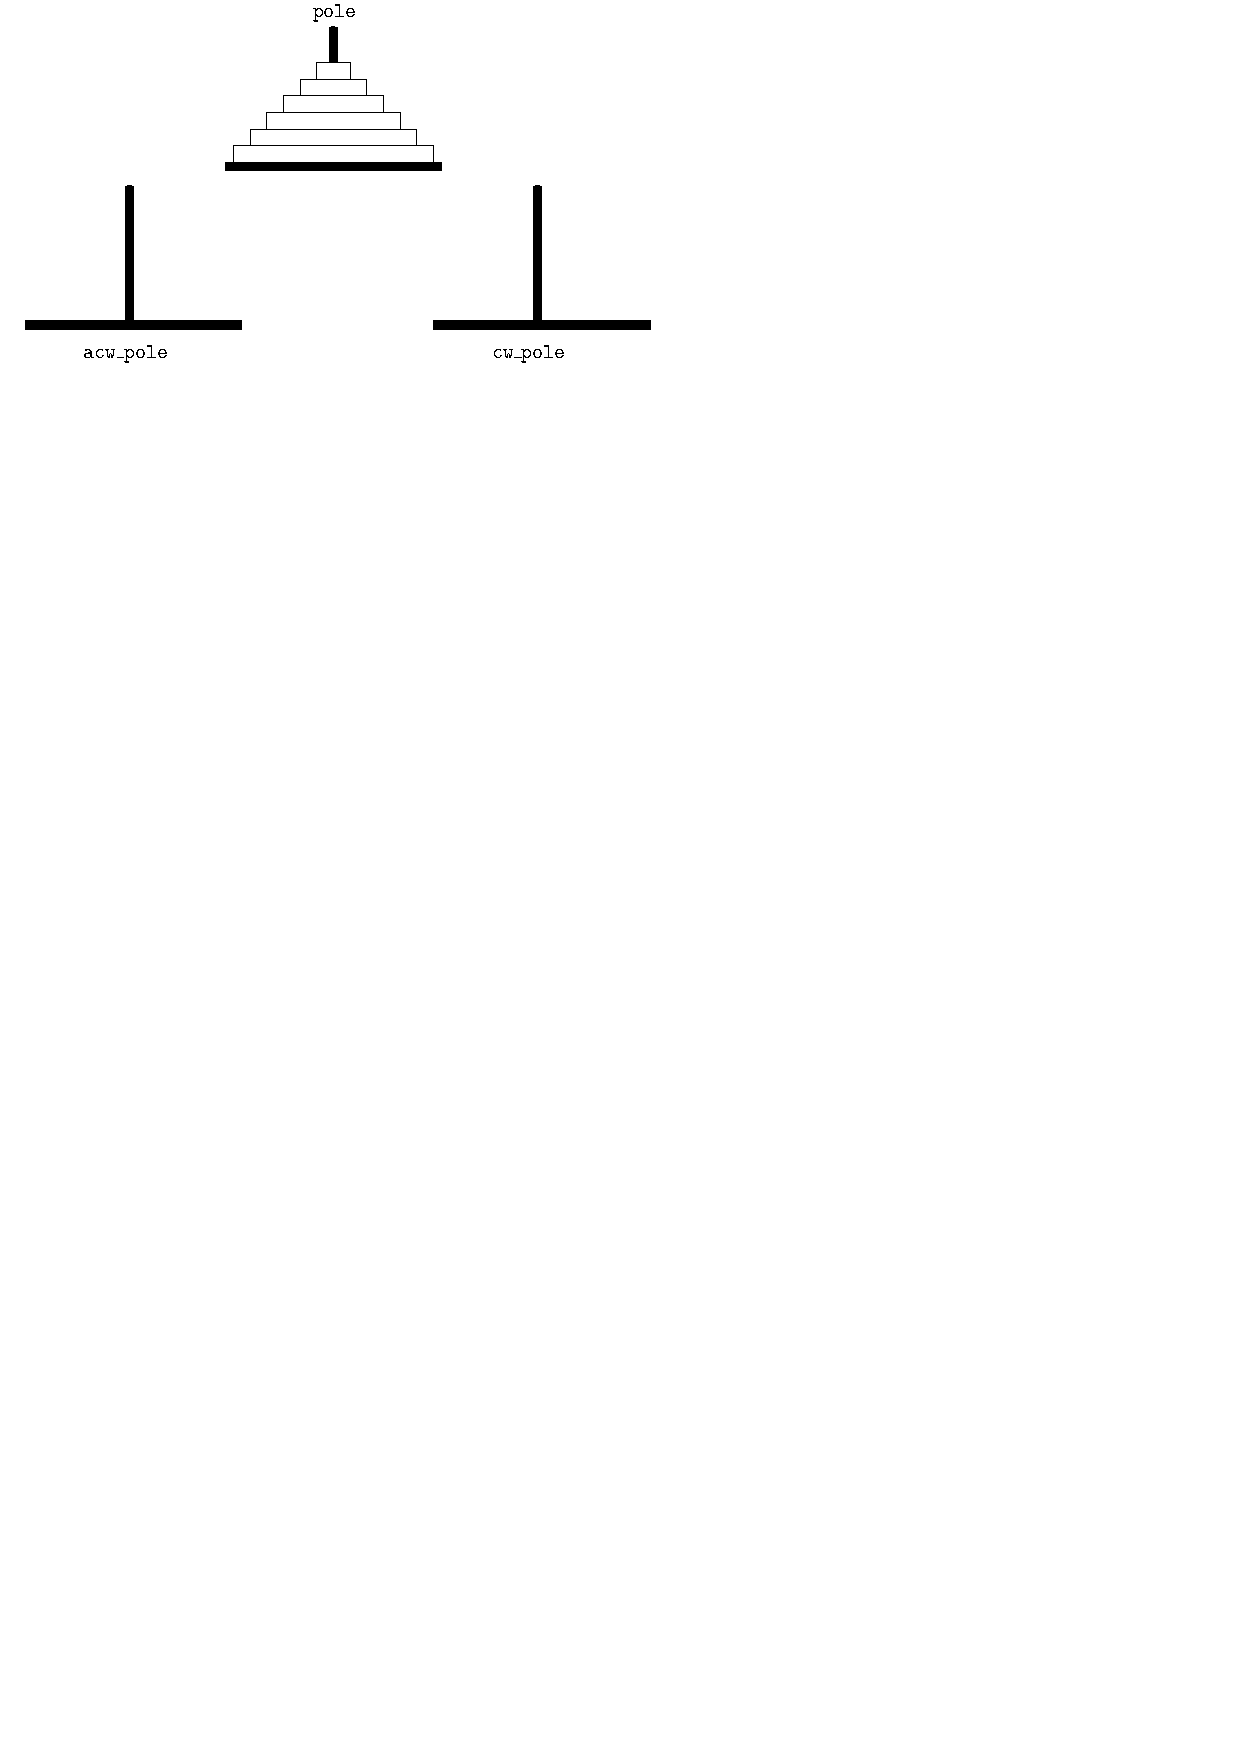
\includegraphics[width=.5\textwidth]{./hanoi2.pdf}
\caption{\label{fig:hanoi2}Tower of Hanoi, pole, clockwise pole, anti-clockwise pole}
\end{figure}


\subsection*{Algorithm development}
\label{sec-2-2}
We can solve the problem recursivley.
\begin{itemize}
\item Base case: There is no disc in the pole.
\item Recursion step: Reduce the size of the tower to $n-1$
discs. Move the tower of top $n-1$ discs to the
anti-clockwise pole. Move the exposed disc ($n$) on the
pole to the clockwise pole. Then, move the tower of $n-1$
discs from anti-clockwise pole to the clockwise pole. This
idea is illustrated in Figure \ref{fig:hanoi5}. Define
\texttt{hanoi()}. Let the function print the sequence of moves on
the \texttt{stdout}.
\end{itemize}
\begin{figure}[htb]
\centering
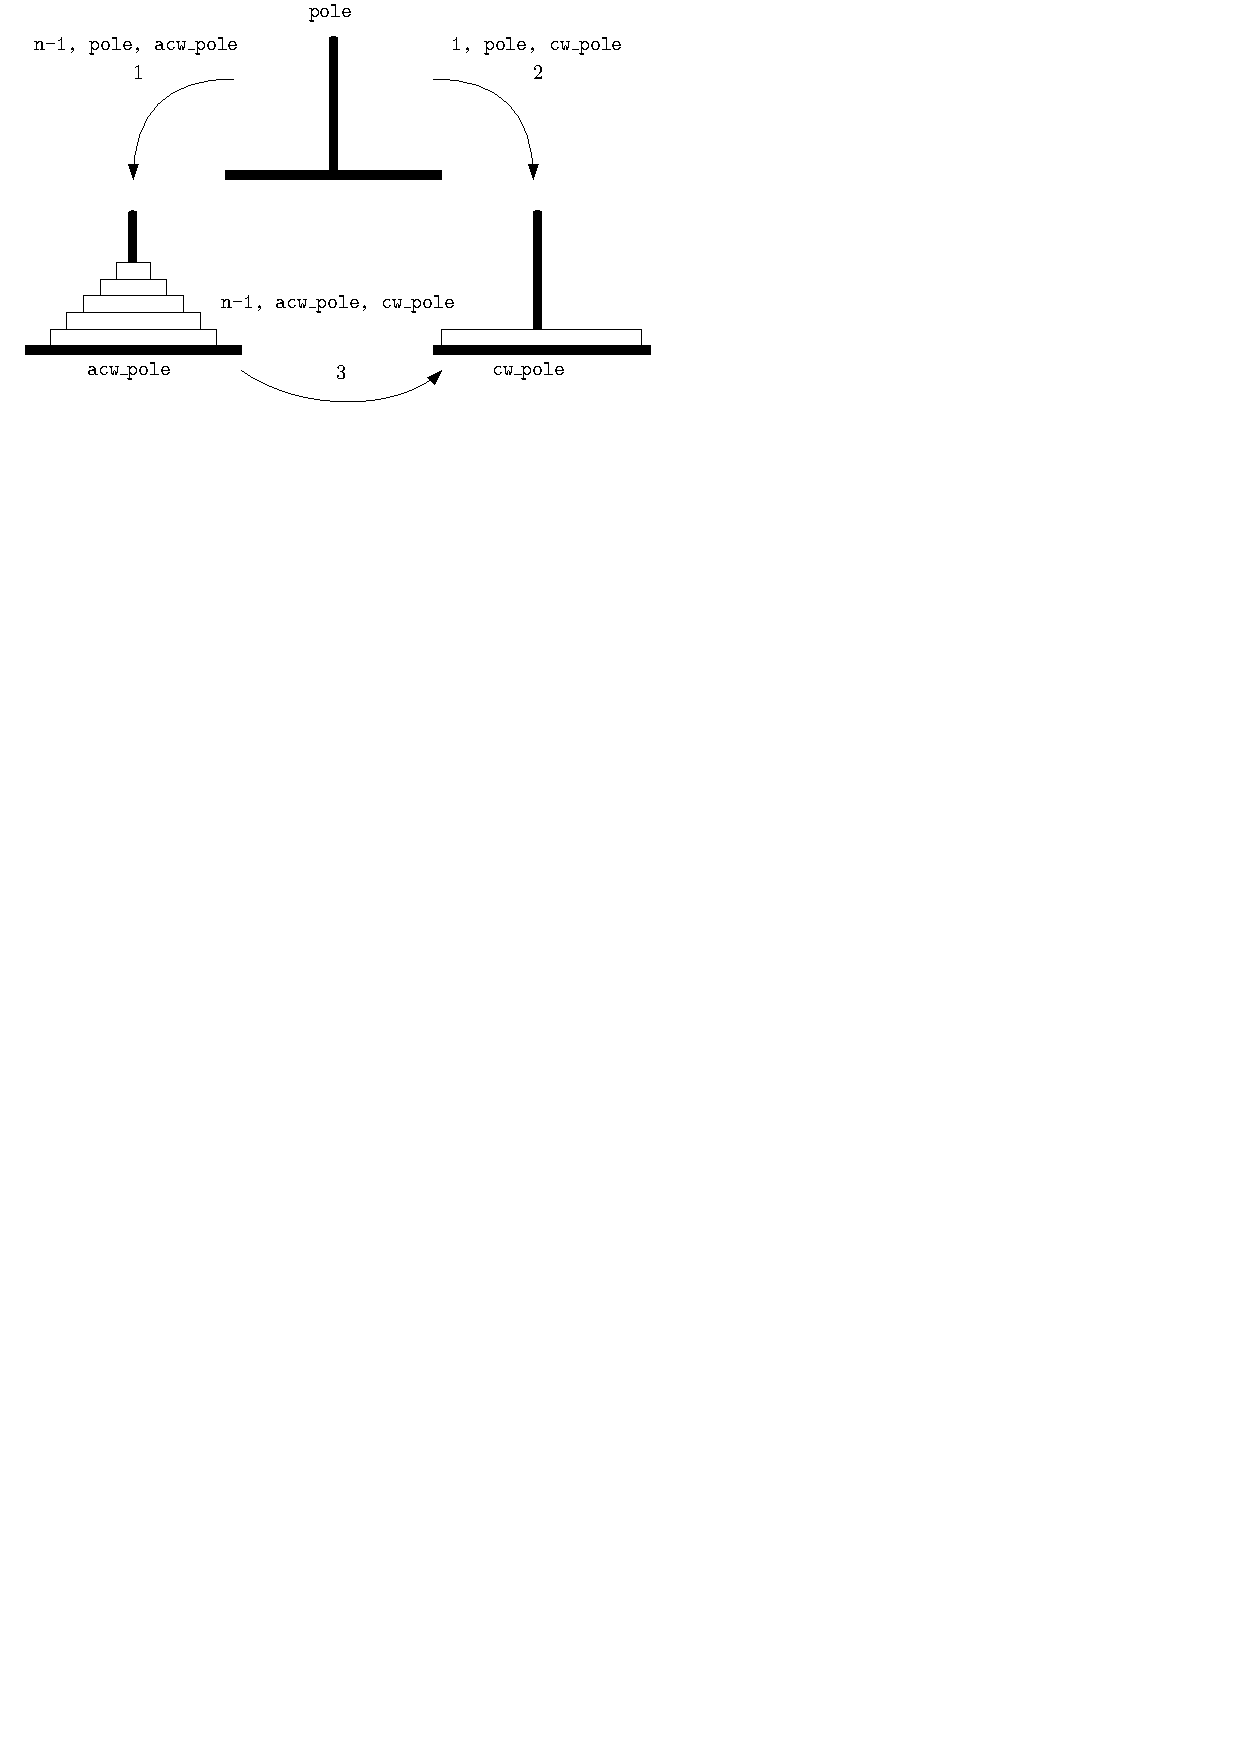
\includegraphics[width=.5\textwidth]{./hanoi5.pdf}
\caption{\label{fig:hanoi5}Tower of Hanoi: move tower in two recursive steps}
\end{figure}
\begin{verbatim}
1: 1 -> 2
2: 1 -> 3
...
\end{verbatim}
\subsection*{Algorithm}
\label{sec-2-3}
\linespread{1}
\begin{verbatim}
move_tower  (n, pole, cw pole, acw pole)
-- pre:  tower of size n on pole, 
--       towers in cw and acw poles are broader than the tower on pole
-- post: tower of size n on cw pole
   if n > 0
      move_tower (n-1, pole, acw pole, cw pole)
      move_disk (pole, cw pole)
      move_tower (n-1, acw pole, cw pole, pole)
\end{verbatim}

\subsection*{Program}
\label{sec-2-4}

\begin{verbatim}
#include<stdio.h>
void move_disc(char from,char to)
{
   printf("move the topmost disc from %c to %c\n",from,to);
}

void move_tower(int n,char pole, char cw_pole,char acw_pole)
{
   if(n>0)
    {
	move_tower(n-1,pole,acw_pole,cw_pole);
	move_disc( pole,cw_pole);
	move_tower(n-1,acw_pole,cw_pole,pole);
    }

}
int main()
{
   int n;

   scanf("%d",&n);
   move_tower(n,'A','B','C');
}
\end{verbatim}
\subsection*{Input}
\label{sec-2-5}
5
\subsection*{Output}
\label{sec-2-6}
\begin{center}
\begin{tabular}{llllllll}
move & the & topmost & disc & from & A & to & B\\
move & the & topmost & disc & from & A & to & C\\
move & the & topmost & disc & from & B & to & C\\
move & the & topmost & disc & from & A & to & B\\
move & the & topmost & disc & from & C & to & A\\
move & the & topmost & disc & from & C & to & B\\
move & the & topmost & disc & from & A & to & B\\
move & the & topmost & disc & from & A & to & C\\
move & the & topmost & disc & from & B & to & C\\
move & the & topmost & disc & from & B & to & A\\
move & the & topmost & disc & from & C & to & A\\
move & the & topmost & disc & from & B & to & C\\
move & the & topmost & disc & from & A & to & B\\
move & the & topmost & disc & from & A & to & C\\
move & the & topmost & disc & from & B & to & C\\
move & the & topmost & disc & from & A & to & B\\
move & the & topmost & disc & from & C & to & A\\
move & the & topmost & disc & from & C & to & B\\
move & the & topmost & disc & from & A & to & B\\
move & the & topmost & disc & from & C & to & A\\
move & the & topmost & disc & from & B & to & C\\
move & the & topmost & disc & from & B & to & A\\
move & the & topmost & disc & from & C & to & A\\
move & the & topmost & disc & from & C & to & B\\
move & the & topmost & disc & from & A & to & B\\
move & the & topmost & disc & from & A & to & C\\
move & the & topmost & disc & from & B & to & C\\
move & the & topmost & disc & from & A & to & B\\
move & the & topmost & disc & from & C & to & A\\
move & the & topmost & disc & from & C & to & B\\
move & the & topmost & disc & from & A & to & B\\
\end{tabular}
\end{center}
% Emacs 24.5.1 (Org mode 8.2.10)
\end{document}
